\documentclass[conference,10pt]{IEEEtran}

\usepackage[utf8]{inputenc}
\usepackage[T1]{fontenc}
\usepackage{amsmath,amssymb,amsfonts}
\usepackage{booktabs}
\usepackage{graphicx}
\usepackage{hyperref}
\usepackage{siunitx}
\usepackage{xcolor}
\usepackage{cite}

\hypersetup{
  colorlinks=true,
  linkcolor=blue!60!black,
  citecolor=blue!60!black,
  urlcolor=blue!60!black
}

\title{VertiRTA: Bare-Metal Fault-Tolerant Run-Time Assurance, Verified Bilingual Contingency Co-Pilot, and License-Clean Active Visual SLZ Perception for Urban Coaxial eVTOLs}

\author{\IEEEauthorblockN{VertiRTA Open-Source Contributors}
\IEEEauthorblockA{Maltepe--Dragos--Kartal Urban Air Mobility Research Testbed, Istanbul, T\"urkiye\\
Repository \& Artifacts: Apache-2.0 Open-Source Release \texttt{v2.0.0} (Baseline \texttt{v1.0.0} Commit \texttt{ef9be75})}}

\begin{document}
\maketitle

\begin{abstract}
Urban coaxial electric vertical take-off and landing (eVTOL) aircraft operating near dense metropolitan airspace must guarantee bounded recovery under rotor, sensor, and battery-sag failures without entrusting flight-critical actuation to unverified neural or language models. We present \textbf{VertiRTA}, an open-source, 100\% Apache-2.0 software-verification and simulation testbed for a 240\,kg coaxial X8 urban eVTOL (\texttt{VertiRTA-X8-240}, 400\,V / 22\,kWh pack) modeled along Istanbul's Maltepe--Dragos--Kartal coastal corridor bounded by real Sabiha G\"ok\c{c}en (\texttt{LTFJ}) and Samand\i ra (\texttt{LTBX}) control zones. VertiRTA enforces an ASTM~F3269-21 Run-Time Assurance (RTA) boundary across three decoupled pillars: (1)~a freestanding, zero-heap C++17 flight core (\texttt{libvertirta\_flight\_core}) pairing 400\,Hz triple-modular-redundant (TMR) IMU voting, coaxial-unblanked f64 INDI+WLS control allocation, Option~B1b active-spin same-arm survival, and a 100\,Hz Hamilton--Jacobi Control Barrier Value Function QP (HJI-CBVF-QP) safety filter; (2)~an asynchronous Turkish/English neuro-symbolic contingency co-pilot combining a $\le 30$-token GBNF grammar, deterministic $\le 32$-node Bounded-STL synthesis, $<12$\,ms Z3 \texttt{QF\_LRA} airspace verification with UNSAT-core repair, zero-heap online STL monitoring, and Split Conformal gating; and (3)~a zero-ShareAlike foundation-distilled active visual Safe Landing Zone (SLZ) stack fusing static-PAPPM \texttt{PIDNet-S} Free-Energy OOD inference into a 1.5625\,MiB cell-local 2.5D Bayesian grid and 5-state inspection orbit. On bare-metal ARM Cortex-M7 (\texttt{-Os}), \texttt{libvertirta\_flight\_core} compiles to 28{,}886\,B Flash, 0\,B static library RAM, 2{,}960\,B worst-case stack DAG, and 0 forbidden heap symbols. Across a live 30{,}000-simulation 6-DOF stratified survival atlas (10{,}000 runs per configuration), \texttt{HJ-CBVF+INDI-WLS} achieves 96.82\% Continued Safe Flight and Landing (CSFL, $n=6{,}500$, $k=207$) versus 44.85\% for HOCBF, and 100.00\% Controlled Emergency Landing (CEL, $n=1{,}500$, $k=0$) versus 0.00\% for stock control allocation, with all 244 failure cliffs published transparently. VertiRTA is strictly a research testbed and makes \emph{no} airworthiness certification or regulatory compliance claim.
\end{abstract}

\begin{IEEEkeywords}
eVTOL, Urban Air Mobility, Run-Time Assurance, ASTM~F3269-21, Control Barrier Value Functions, Fault-Tolerant Control, Signal Temporal Logic, Safe Landing Zone Perception.
\end{IEEEkeywords}

\section{Introduction and Scope Boundaries}
\label{sec:intro}

Deploying electric vertical take-off and landing (eVTOL) aircraft over coastal urban corridors introduces a tight coupling between propulsion fault tolerance, high-voltage battery voltage sag, controlled-airspace geofencing, and emergency landing site selection. In safety-critical aerospace engineering, however, combining deterministic flight-control kernels with modern neural perception or Large Language Models (LLMs) frequently creates two failure modes in academic prototypes: (i)~architectural entanglement, where untrusted Python or neural workloads share threads, memory, or actuation paths with control loops, and (ii)~regulatory overclaiming, where modest simulation campaigns are misframed as DO-178C, EASA \texttt{SC-VTOL-02}, or \texttt{SORA 2.5} compliance.

\textbf{Explicit Non-Certification Disclaimer:} VertiRTA (\texttt{libvertirta\_flight\_core}, \texttt{libvertirta\_rta\_companion}, \texttt{vertirta\_copilot}, \texttt{vertirta\_stl\_monitor}, and \texttt{vertirta\_slz\_bayes}) is an open-source research, simulation, and software-verification testbed only. It is \emph{not} a certified airborne product, does \emph{not} claim DO-178C, DO-254, ARP4754B, EASA \texttt{SC-VTOL-02}, \texttt{SORA 2.5}, or SHGM \texttt{SHT-\.IHA} compliance, and does \emph{not} substitute for bare-metal real-time operating system (RTOS) Worst-Case Execution Time (WCET) certification evidence~\cite{easa_scvtol_2024,easa_sora25_2026,shgm_sht_iha_2026}.

Our architecture is anchored to a realistic, physically closed reference vehicle and metropolitan operational domain:
\begin{itemize}
  \item \textbf{Reference Airframe (\texttt{VertiRTA-X8-240}):} A $m=240.0$\,kg coaxial X8 multicopter ($W=2{,}353.6$\,N, four booms of radius $L=1.35$\,m, eight rotors of radius $R=0.75$\,m with upper/lower coaxial spacing $0.35$\,m) powered by a 112S12P $400.0$\,V / $22.0$\,kWh 1-RC Th\'evenin NMC811 battery pack ($R_0=0.1363\,\Omega$, $R_1=0.0840\,\Omega$, $C_1=300$\,F) and voltage-headroom windings ($K_{e,\text{bus}}=1.36$\,V$\cdot$s/rad) preserving two-arm hover thrust-to-weight $\ge 1.12$ down to $338$\,V terminal sag.
  \item \textbf{Istanbul Coastal Operational Domain (\texttt{ODD.yaml}):} A Maltepe--Dragos--Kartal coastal corridor anchored at Kartal Coastal Vertiport ($40.8860^\circ$\,N, $29.1880^\circ$\,E, $12.0$\,m AMSL; EGM2008 geoid undulation $N=+36.7$\,m, yielding $48.7$\,m HAE). To respect the real AIP T\"urkiye Sabiha G\"ok\c{c}en (\texttt{LTFJ}) 5\,NM + NW \texttt{J1}/\texttt{J2} control zone (pinch at $29.19212^\circ$\,E) and Samand\i ra (\texttt{LTBX}) military CTR, nominal corridor operations are strictly bounded west of $29.1900^\circ$\,E and enforced as hard deterministic barriers.
  \item \textbf{Strict ASTM~F3269-21 Simplex Isolation:} Untrusted complex functions---both the bilingual TR/EN contingency co-pilot (Pillar~2) and foundation-distilled visual SLZ perception (Pillar~3)---execute outside the deterministic flight and RTA core with zero closed-loop actuation authority and $0\,\mu$s jitter impact on the 100\,Hz RTA thread~\cite{astm_f3269_2021}.
\end{itemize}

\textbf{Contributions:} (1)~A bare-metal verified zero-heap C++17 flight core and 100\,Hz HJI-CBVF-QP companion with automated 4-tier determinism gates; (2)~a live 30{,}000-simulation 6-DOF stratified survival atlas isolating CSFL from same-arm CEL denominators with a zero-cherry-picking failure cliff ledger; (3)~an asynchronous neuro-symbolic TR/EN contingency architecture pairing compact GBNF decoding, Z3 \texttt{QF\_LRA} airspace proofs, zero-heap STL monitoring, and Split Conformal gating; (4)~a license-clean, zero-ShareAlike visual SLZ perception and active inspection pipeline; and (5)~an audit-linted, manifest-driven reproducible paper workflow separating verified local artifacts from explicitly labeled pending cloud/SITL campaigns.

\section{Pillar 1: Bare-Metal Flight Core and HJI-CBVF-QP Safety Filter}
\label{sec:pillar1}

\subsection{400\,Hz Coaxial INDI+WLS, Unblanking, and Active-Spin CEL}

Pillar~1 separates hardware-portable inner-loop control (\texttt{libvertirta\_flight\_core}, freestanding C++17 compiled with \texttt{-fno-exceptions -fno-rtti -ffp-contract=off -fno-fast-math}) from 100\,Hz companion-computer safety filtering (\texttt{libvertirta\_rta\_companion}, C++20). At 400\,Hz, three asynchronous-safe IMU channels pass through a triple-modular-redundant (TMR) median/chi-squared cross-monitor (\texttt{TmrVoter}) isolating hardover, bias-ramp, or freeze faults within $\le 20$\,ms, directly aligned with continuous fly-by-wire latent-fault monitoring principles in EASA \texttt{MOC-5 VTOL.2300}~\cite{easa_moc5_2026}.

Rotor thrust effectiveness explicitly captures coaxial rotor-wake interference~\cite{leishman_principles_2006}: under nominal hover, lower rotors $\{4,5,6,7\}$ operate inside upper-rotor $\{0,1,2,3\}$ downwash with efficiency $\eta_{\text{coax},0}=0.85$. When an upper rotor $i\in\{0..3\}$ fails, \texttt{CoaxEffectiveness::build\_B} unblanks its coaxial lower partner $i+4$ to $\eta_t=1.0$ ($+17.6\%$ thrust recovery, $676.1\to 795.4$\,N at $400$\,V) while scaling per-rotor speed ceilings dynamically from live 1-RC Th\'evenin terminal voltage $V_{\text{term}}$. A dual-channel fault detection and isolation observer (\texttt{MotorFdiObserver}) fuses ESC RPM innovation ($<60$\,ms) and sensorless 4-DOF wrench residuals ($<85$\,ms, immune to $45$\,N$\cdot$m coastal gust moments) to classify five discrete flight regimes: \texttt{NOMINAL}, \texttt{SINGLE\_LOSS} (1M), \texttt{CROSS\_DUAL} (2M-Cross), \texttt{SAME\_ARM\_ACTIVE\_SPIN} (2M-SameArm), and \texttt{CRITICAL\_DESCENT}.

For 4-DOF-controllable regimes (\texttt{NOMINAL}, 1M, 2M-Cross), an Incremental Nonlinear Dynamic Inversion loop drives an active-set Weighted Least Squares allocator (\texttt{wls\_alloc\_8x4\_f64}) assembled strictly in IEEE-754 \texttt{double} precision to eliminate single-precision Cholesky rank-deficiency~\cite{smeur_indi_wls_2020}. When a same-arm coaxial pair fails (e.g., M0+M4), roll/pitch torque along the failed-boom diagonal becomes unilateral and 4-DOF hover is physically impossible. Rather than allowing roll capsize, VertiRTA latches an irreversible \texttt{LATCHED\_CEL} mode in $\le 1$ tick ($2.5$\,ms), unloading the opposite boom and stabilizing reduced attitude around a controlled Option~B1b flat spin at $|\Omega_z|=2.2$\,rad/s~\cite{mueller_relaxed_hover_2014}, compensated by actuator-lag phase lead $\Delta\psi=\arctan(\Omega_z\tau_{\text{up}})\approx 10.6^\circ$ ($\tau_{\text{up}}=0.085$\,s). Because uncontrolled passenger yaw is incompatible with passenger-grade CSFL, same-arm dual failure is strictly separated from the CSFL statistical pool and evaluated solely as last-resort Controlled Emergency Landing (CEL) survivability.

\subsection{100\,Hz HJI-CBVF-QP Safety Filter and 4-Thread Lock-Free Transport}

At 100\,Hz, \texttt{CbvfSafetyFilter} evaluates a memory-mapped, SHA-256-verified 4D Hamilton--Jacobi Control Barrier Value Function lookup table (\texttt{MmapCbvf4DLut}, \texttt{VRTALUT1}) indexed over horizontal/vertical separation, closing velocity, and active flight regime~\cite{choi_cbvf_2021}. Conservatively subtracting the grid discretization margin $\epsilon_{\text{grid}}$ from quadrilinearly interpolated $V(x)$ and $\nabla V(x)$, the filter enforces the barrier-value inequality
\begin{equation}
  \nabla_x V(x)^\top f(x) + \nabla_x V(x)^\top g(x)\,u \;\ge\; -\gamma_{\text{cbvf}}\bigl(V(x)-\epsilon_{\text{grid}}\bigr) - \delta,
  \label{eq:cbvf_qp}
\end{equation}
across static obstacles, 3.094\,MiB robocentric Euclidean Signed Distance Field (ESDF) cells, 64 thin-wire capsules, 16 Kalman-tracked intruders, and hard \texttt{LTFJ}/\texttt{LTBX} CTR walls via a zero-heap embedded C99 dual active-set QP solver (\texttt{StaticDaqpSolver<5,32>}, 5{,}888\,B static workspace, zero recursion)~\cite{arnstrom_daqp_2022}. Tall CTR walls enforce horizontal braking without climb-over hallucination, opposing-gradient clutter inflates clearance by $+1.5$\,m, and any infeasible QP or $V<-0.25$\,m triggers closed-form worst-case HJI braking $u^*_{\text{HJ}}$. During \texttt{LATCHED\_CEL}, the 4-DOF QP is bypassed in favor of a 2D flat-spin vertical braking LUT (\texttt{Cel2DLut}).

Between ROS~2 Jazzy and PX4~v1.16 (\texttt{px4-ros2-interface-lib}), \texttt{vertirta\_rta\_node} isolates the 100\,Hz \texttt{SCHED\_FIFO} RTA thread using cache-line-aligned (\texttt{alignas(64)}) lock-free single-producer single-consumer (SPSC) ring buffers and atomic-word Seqlock snapshots, verified under ThreadSanitizer across $10^6+$ concurrent 4-thread operations with zero data races and zero torn reads. An irreversible \texttt{cel\_latched\_} flag inside \texttt{VertiRtaMode} guarantees that once CEL engages, PX4 cannot unlatch back to position control in flight.

% Auto-generated by docs/paper/scripts/generate_latex_tables.py -- DO NOT HAND-EDIT.
% Source manifest: metrics_manifest.json

\begin{table}[t]
\centering
\caption{Pillar 1 Bare-Metal Structural Footprint, Isolation, and Execution Determinism (\texttt{libvertirta\_flight\_core} + \texttt{rta\_companion}).}
\label{tab:tier1_determinism}
\scriptsize
\begin{tabular}{@{}lll@{}}
\toprule
\textbf{Metric} & \textbf{Measured / Status} & \textbf{Gate / Scope} \\
\midrule
Cortex-M7 Flash (\texttt{.text+.data}) & 28{,}886\,B & Budget $<262{,}144$\,B ($256$\,KiB) \\
Cortex-M7 Static Library RAM & 0\,B & Caller-owned static arenas ($<128$\,KiB) \\
Cortex-M7 Max Static Stack Frame & 1496\,B & Limit $\le 4{,}096$\,B ($0$ dynamic) \\
Cortex-M7 Max Call-Graph Stack DAG & 2960\,B & Limit $\le 16{,}384$\,B ($0$ recursion) \\
Host x86\_64 Stack Frame / DAG & 2112\,B / 5280\,B & All 8 \texttt{flight\_core} modules \\
Forbidden Heap Symbols (\texttt{nm}) & 0 & x86\_64 \& Cortex-M7 + \texttt{--wrap=malloc} \\
ASTM F3269-21 Core Isolation & 0 violations & 37 core files scanned \\
Tier-3 \texttt{THREAD\_CPUTIME} p50 / p99 / p99.9 & 1.24 / 1.90 / 11.57\,$\mu$s & Local WSL2 x86\_64 ($100\text{k}$ ticks) \\
Tier-4 \texttt{MONOTONIC\_RAW} p50 / p99 / p99.9 & 0.54 / 0.95 / 1.59\,$\mu$s & Steal 0.0\% (CLEAN) \\
Cloud ARM64 (\texttt{ubuntu-24.04-arm}) Cross-ISA & PASS (Cobalt 100: p99 0.736 us, 0.0 cross-ISA diff) & Azure Cobalt 100 GitHub Actions CI \\
Tier-3 Callgrind Work Units (ARM64 / x86\_64) & 604{,}543 / 723{,}331\,Ir/tick & Budget $\le 1{,}200{,}000$\,Ir/tick \\
\bottomrule
\end{tabular}
\end{table}

\begin{table*}[t]
\centering
\caption{Pillar 1 Tier-1 6-DOF Stratified Survival Envelope Atlas \& A/B Ablation (Isolated CSFL vs.\ Same-Arm CEL Denominators; One-Sided 95\% Clopper-Pearson Upper Failure Bounds).}
\label{tab:tier1_atlas}
\scriptsize
\begin{tabular}{@{}lcccc@{}}
\toprule
\textbf{Controller / Filter Config} & \textbf{CSFL Pass (S2+S3+S5)} & \textbf{CSFL CP95 Upper} & \textbf{CEL Pass (S4 Same-Arm)} & \textbf{CEL CP95 Upper} \\
\midrule
\textbf{HJ-CBVF + INDI-WLS} & 96.82\% ($n=6500$) & 3.57\% & 100.00\% ($n=1500$) & 0.20\% \\
HOCBF + INDI-WLS & 44.85\% & 56.17\% & 100.00\% & 0.20\% \\
HJ-CBVF + Stock CA & 96.82\% & 3.57\% & 0.00\% & 100.00\% \\
\bottomrule
\end{tabular}

\vspace{2pt}
{\tiny CSFL failures $k=207$; CEL failures $k=0$; Total cliff ledger entries: 244 / 10{,}000; 30{,}000 total 6-DOF sims in 77.32\,s; Zero-failure $10^{-9}$/FH horizon: 2{,}995{,}732{,}273\,FH; Tier-2 PX4/Gz 1k: Pending (PX4/Gz SITL); Tier-3 EGL LiDAR 50: Pending (PX4/Gz SITL).}
\end{table*}

\begin{table}[t]
\centering
\caption{Pillars 2 \& 3 Verified Architectural Locks and Pending Cloud/GPU Evaluation Campaigns (Zero Fabricated Metrics).}
\label{tab:pillars23_status}
\scriptsize
\begin{tabular}{@{}lll@{}}
\toprule
\textbf{Subsystem / Metric} & \textbf{Value / Status} & \textbf{Evidence Tier} \\
\midrule
Pillar 2: Conformal Quantile Level $q_{\text{lvl}}$ & 0.955 & Verified lock \\
Pillar 2: Compact GBNF DSL Token Cap & 30 tokens & Verified lock \\
Pillar 2: Bounded-STL AST Node Cap & 32 nodes & Verified lock \\
Pillar 2: Z3 \texttt{QF\_LRA} Timeout Cap & 12\,ms & Verified lock \\
Pillar 2: HV Pack Contract (Voltage / Energy) & 400.0\,V / 22.0\,kWh & Locked to \texttt{vehicle\_x8\_240.yaml} \\
Pillar 2: Unsafe Command Rejection Rate & Pending (Colab G4) & Deferred training/eval \\
Pillar 2: Conformal Empirical Coverage & Pending (Colab G4) & Deferred training/eval \\
Pillar 2: Human-Audited VertiBench-TR/EN & Pending (Colab G4) & Deferred training/eval \\
Pillar 3: Cell-Local 2.5D SLZ Grid Footprint & 1.5625\,MiB & Verified lock \\
Pillar 3: Pad Footprint Disk ($R_{\text{SLZ}}\ge 5$\,m) & 317 cells & Verified lock \\
Pillar 3: Geometry Gates ($R_{\min} / \theta_{\max} / \sigma_{z,\max}$) & 5.0\,m / 8.0$^\circ$ / 0.15\,m & Enforced by \texttt{SlzBeliefGrid} \\
Pillar 3: Perception Staleness Contract & 250\,ms & Verified lock \\
Pillar 3: Active Orbit Safe Touchdown & Pending (Colab G4) & Deferred GPU campaign \\
Pillar 3: Active Orbit False-Commit Rate & Pending (Colab G4) & Deferred GPU campaign \\
Pillar 3: Zero-Shot AeroScapes mIoU & Pending (Colab G4) & Deferred GPU campaign \\
Pillar 3: Free-Energy OOD AUROC & Pending (Colab G4) & Deferred GPU campaign \\
Pillar 3: Local WSL2 GTX 1650S Peak VRAM & Pending (WSL2 GTX 1650S) & Deferred GPU campaign \\
Pillar 3: Local WSL2 3/3 Smoke Touchdowns & Pending (WSL2 GTX 1650S) & Deferred GPU campaign \\
\bottomrule
\end{tabular}
\end{table}


\section{Pillar 2: Verified Bilingual TR/EN Contingency Co-Pilot}
\label{sec:pillar2}

Human operators and passengers during urban eVTOL contingencies frequently communicate under workload in Turkish, English, or code-switched phrases (e.g., requesting an immediate diversion to a specific coastal pad or questioning remaining energy). Pillar~2 (\texttt{v2.0.0-alpha}) integrates an asynchronous ($0.5$--$1$\,Hz) neuro-symbolic co-pilot positioned strictly at EASA AI Level~1B/2A advisory scope (DAL~E, zero closed-loop actuation authority)~\cite{easa_ai_cp_2026}.

\subsection{Compact $\le 30$-Token GBNF Decoding and Deterministic STL Synthesis}

Unconstrained LLM generation of Signal Temporal Logic (STL) formulas suffers from syntax failures, high latency under single-digit BPE tokenization, and prompt-injected reasoning loops (e.g., adversarial \texttt{/think} or \texttt{<think>} probes). VertiRTA constrains Apache-2.0 \texttt{Qwen3-4B}/\texttt{8B} inference inside \texttt{VertiLlamaEngine} (\texttt{libllama}) via eager GBNF grammar enforcement (\texttt{vertirta\_dsl\_v1.gbnf}) with \texttt{enable\_thinking=False} to a strict two-line ASCII domain-specific language of $\le 30$ tokens (six action kinds: \texttt{DIVERT\_SLZ}, \texttt{INSPECT\_SLZ}, \texttt{ABORT\_RETURN}, \texttt{HOLD\_LOITER}, \texttt{REQUEST\_CLARIFICATION}, and \texttt{REJECT\_UNSAFE}, paired with \texttt{LNG=\{TR,EN,MIX\}} and \texttt{MOD=\{BRIEF,REJECT,CLARIFY\}}).

A zero-allocation parser (\texttt{parse\_compact\_dsl}) rejects malformed tokens or trailing bytes, and \texttt{synthesize\_canonical\_stl} deterministically expands each validated AST into a $\le 32$-node Bounded-STL specification~\cite{donze_stl_2010}, e.g., for diversions:
\begin{equation}
  \phi_{\text{div}} = \mathbf{G}_{[0,t_c]}\!\bigl(\text{AGL}\!\ge\!h_{\min} \wedge \neg\text{CTR}\bigr) \wedge \mathbf{G}_{[0,\eta]}\!\bigl(\text{SoC}\!\ge\!12\%\bigr) \wedge \mathbf{U}_{[0,\eta]}\!\bigl(\text{AGL}\!\ge\!h_f,\text{reach}(\text{tgt})\bigr).
  \label{eq:stl_divert}
\end{equation}
Online trajectory compliance is monitored in pure zero-heap C++20 (\texttt{vertirta\_stl\_monitor}, $<1$\,ms/tick) using a wraparound-safe \texttt{FixedMonotonicWedge<601>} ring buffer that evicts expired heads prior to tail insertion, preventing false-positive robustness wrap corruption.

\subsection{Z3 \texttt{QF\_LRA} Airspace Verification, UNSAT Repair, and Split Conformal Gating}

Before any proposal crosses the asynchronous ROS~2 Action (\texttt{/vertirta/execute\_contingency}) to \texttt{VertiRtaExecutor}, a native C++ Z3 \texttt{QF\_LRA} verifier~\cite{demoura_z3_2008} checks corridor segments against real \texttt{LTFJ}/\texttt{LTBX} 3D airspace prisms, up to four dynamic NFZs with distinct named assertions (preventing Z3 tracker collisions), battery reserve floors ($12\%$ on the $400$\,V/$22$\,kWh pack), and SLZ safety thresholds under a strict \texttt{rlimit}=250{,}000 / $12$\,ms timeout (fail-closed on \texttt{unknown}). Upon \texttt{UNSAT}, an 8-priority deterministic UNSAT-core repair loop substitutes the highest-ranked Z3-SAT alternate or safe loiter and renders grounded bilingual feedback verified by a Numeric Grounding Gate.

To prevent overconfident guesses under ambiguous or noisy speech commands, a \texttt{KnowNo}-style Split Conformal Prediction gate~\cite{ren_knowno_2023} calibrated at $n_{\text{cal}}=200$, $\alpha=0.05$ ($q_{\text{lvl}}=0.955$) retains a prediction set $\mathcal{C}_{\text{safe}}$ of Z3-verified actions. When $|\mathcal{C}_{\text{safe}}|\neq 1$, the co-pilot triggers active clarification (\texttt{HOLD\_LOITER} + \texttt{REQUEST\_CLARIFICATION}) unless remaining loiter SoC margin drops below $5.0\%$, in which case a liveness override immediately commits the Rank-1 Z3-SAT SLZ to prevent battery-depletion deadlock. Training and evaluation pipelines (\texttt{VertiBench-TR/EN}, strict $<0.15$ 5-gram Jaccard split separation, SFT$\to$Z3-GRPO with \texttt{spawn}-isolated Z3 reward pools) are fully implemented and unit-tested; full Colab G4 \texttt{Qwen3-8B} training and human-audited benchmark execution are explicitly tracked as \texttt{Pending (Colab G4)} in Table~\ref{tab:pillars23_status}.

\section{Pillar 3: License-Clean Active Visual SLZ Perception}
\label{sec:pillar3}

Pre-mapped vertiports may become obstructed by transient vehicles, construction tarps, or crowds during an unscheduled diversion. Pillar~3 (\texttt{v2.0.0}) replaces blind DEM lookup with a license-clean active visual SLZ pipeline plugged into Plan~1A's \texttt{ISlzPriorProvider} interface via lock-free SPSC queues in \texttt{vertirta\_perception\_node}, preserving $0\,\mu$s jitter on the 100\,Hz RTA kernel and flagging frames older than $250$\,ms as stale.

\subsection{Zero-ShareAlike License Gate and Static-PAPPM \texttt{PIDNet-S}}

Many aerial segmentation datasets carry ShareAlike, non-commercial, or export-restricted licenses incompatible with permissive industrial robotics deployment. Pillar~3 enforces a programmatic startup \texttt{verify\_training\_manifest} gate restricting training exclusively to five permissive sources: \texttt{FLAIR-1} (\texttt{etalab-2.0}), a programmatic 41/100 \texttt{OpenEarthMap} whitelist (\texttt{CC~BY~4.0} + \texttt{DL-DE-BY-2.0} only), \texttt{FloodNet-Supervised v1.0} (\texttt{CDLA-Permissive-1.0}), \texttt{SkyScenes} (\texttt{MIT}, filtered via depth-derived surface normals $|n_z|<0.85$ so vertical building facades are never mislabeled as flat roofs), and an author-generated 8{,}000-frame Gazebo Harmonic EGL Istanbul dataset built over Copernicus GLO-30 procedural blocks with strict OSM \texttt{ODbL} exclusion. Restricted datasets and backbones (\texttt{RescueNet}, \texttt{LoveDA}, \texttt{DINOv3}, \texttt{SegFormer}, \texttt{Depth-Anything-V2-Large/Base/Giant}) are hard-banned, while \texttt{AeroScapes}, \texttt{ICG}, and \texttt{UAVScenes} are quarantined strictly to zero-shot evaluation.

For real-time onboard inference, frozen Apache-2.0 teachers (\texttt{DINOv2-ViT-L/14}~\cite{oquab_dinov2_2024} and \texttt{Depth Anything V2 Small}~\cite{yang_depthanythingv2_2024}) distill into a static-PAPPM \texttt{PIDNet-S} student~\cite{xu_pidnet_2023} ($512\times 512$ input, zero dynamic \texttt{AdaptiveAvgPool2d} layers for deterministic ONNX Opset~17+ / TensorRT export) equipped with a unit-normal prediction head and a Helmholtz Free-Energy out-of-distribution (OOD) score~\cite{liu_energy_ood_2020}:
\begin{equation}
  E_{\text{free}}(x) = -T_{\text{ood}}\log\sum_{c=0}^{4}\exp\!\left(\frac{z_c(x)}{T_{\text{ood}}}\right), \quad T_{\text{ood}}=1.0.
  \label{eq:free_energy}
\end{equation}

\subsection{Cell-Local 2.5D Bayesian Grid and 5-State Active Inspection Orbit}

Rather than computing world-frame covariance $\Sigma=M/N-\bar{p}\bar{p}^\top$ in \texttt{float32}---which suffers catastrophic cancellation at Maltepe ENU offsets ($\pm 3{,}500$\,m)---our C++20 \texttt{SlzBeliefGrid} ($160\times 160$ cells at $0.5$\,m resolution, exact $1.5625$\,MiB static footprint) accumulates cell-local displacements $\delta p = p_W - c_{ij}$, rejects sparse cells ($<12$ points), and verifies candidate pads over the full $317$-cell disk ($R_{\text{SLZ}}\ge 5.0$\,m, slope $\theta\le 8.0^\circ$, roughness $\sigma_z\le 0.15$\,m, step $\le 0.25$\,m). To prevent additive Bayesian precision collapse when an OOD hazard (e.g., an unseen tarp) appears over a previously clean roof, \texttt{SlzBeliefGrid} enforces an explicit OOD variance floor and precision cap whenever normalized free energy exceeds $\tau_{\text{ood}}$.

A deterministic 5-state \texttt{ActiveInspectionPolicy} (\texttt{CANDIDATE\_EVAL}, \texttt{APPROACH\_ORBIT}, \texttt{ACTIVE\_INSPECT\_ORBIT}, \texttt{COMMIT\_TOUCHDOWN}, \texttt{REJECT\_DIVERT\_NEXT}) commands a tilted 2-axis kinematic gimbal (avoiding nadir $80^\circ$-HFOV pad-edge clipping) and arms its $12.0$\,s inspection timer only after descending into orbit altitude, consuming $\approx 0.614\%$ SoC per $12$\,s orbit on the $22$\,kWh pack. Full Colab G4 distillation/60-seed EGL ablation and local WSL2 \texttt{GTX 1650 SUPER} ($<300$\,MB VRAM) FP32/FP16 profiling scripts are implemented and unit-tested, with live GPU measurements explicitly tracked as \texttt{Pending (Colab G4)} / \texttt{Pending (WSL2 GTX 1650S)} in Table~\ref{tab:pillars23_status}.

\section{Experimental Results and Honest Failure Cliff Analysis}
\label{sec:results}

All Pillar~1 evidence reported in Tables~\ref{tab:tier1_determinism} and~\ref{tab:tier1_atlas} was executed live on commit \texttt{ef9be75} (WSL2 Ubuntu x86\_64, \texttt{g++ 15.2.0 -O2} strict IEEE-754 + \texttt{arm-none-eabi-g++ 14.2.1 -Os} Cortex-M7) and stored as SHA-256-indexed artifacts under \texttt{artifacts/v1.0.0/}.

\subsection{Bare-Metal Footprint, Zero-Heap Proof, and 4-Tier Determinism}

As summarized in Table~\ref{tab:tier1_determinism}, bare-metal ARM Cortex-M7 (\texttt{STM32H753 FPv5-D16}) compilation of \texttt{libvertirta\_flight\_core.a} across all 11 object modules occupies $28{,}886$\,B Flash ($11.0\%$ of the $256$\,KiB budget) and $0$\,B static library RAM, with $0$ forbidden heap symbols verified by both \texttt{arm-none-eabi-nm} and host \texttt{nm} plus link-time \texttt{-Wl,--wrap=malloc/calloc/realloc} traps. Static call-graph analysis (\texttt{-fstack-usage -fcallgraph-info=su,da}) bounds worst-case Cortex-M7 frame size at $1{,}496$\,B ($77$ functions, $0$ dynamic) and worst-case DAG stack depth at $2{,}960$\,B ($98$ nodes, $0$ recursion; worst chain \texttt{IndiWlsController::step\_400hz} $\to$ \texttt{wls\_alloc\_8x4\_f64}). Architecture isolation scanning confirms $0$ AI/ROS/Python/PROJ dependencies across all $37$ core files.

On Tier-2 deterministic replay of the golden $20.0$\,s ($2{,}000$-frame, $512{,}128$\,B, $1{,}400$ CEL-latched frames) corridor fault fixture \texttt{corridor\_faults.vrta}, repeated x86\_64 and live GitHub Actions \texttt{ubuntu-24.04-arm} (Azure Cobalt~100 / Neoverse~N2) replays achieve exact 0-ULP SHA-256 bit-identity both within each architecture and cross-ISA (\texttt{mode\_divergences=0}, \texttt{max\_abs\_diff=0.0} across all $2{,}000$ frames). On local WSL2 x86\_64 Release \texttt{vertirta\_bench\_cli} (full 100\,Hz CBVF-QP + 400\,Hz INDI-WLS tick with LUTs loaded), Tier-3 \texttt{CLOCK\_THREAD\_CPUTIME\_ID} ($100{,}000$ ticks) measures $1.24\,\mu$s p50 / $1.90\,\mu$s p99 / $11.57\,\mu$s p99.9, and Tier-4 \texttt{CLOCK\_MONOTONIC\_RAW} ($50{,}000$ ticks) measures $0.54\,\mu$s p50 / $0.95\,\mu$s p99 / $1.59\,\mu$s p99.9 at $0.0\%$ steal; live cloud \texttt{ubuntu-24.04-arm} (Cobalt~100, $20{,}000$ ticks) measures $0.720\,\mu$s p50 / $0.736\,\mu$s p99 / $0.864\,\mu$s p99.9 at $0.0\%$ steal (\texttt{CLEAN}) and $604{,}543$\,Ir/tick under Valgrind Callgrind ($723{,}331$\,Ir/tick on \texttt{ubuntu-24.04} x86\_64)---over $10{,}000\times$ inside the $10{,}000\,\mu$s outer-loop frame period. Per our WCET scope caveat, Linux user-space timings are CI regression telemetry only and are \emph{not} RTOS WCET certification evidence.

\subsection{Live 30{,}000-Simulation 6-DOF Survival Atlas and A/B Ablation}

To quantify fault-recovery boundaries without cherry-picking, we executed the full Tier-1 6-DOF stratified Latin Hypercube Sampling (LHS) atlas (\texttt{seed=20261122}, $10{,}000$ runs across strata S1--S6) across three configurations totaling $30{,}000$ closed-loop 6-DOF simulations in $77.32$\,s wall-clock time (Table~\ref{tab:tier1_atlas}, Figs.~\ref{fig:heatmap}--\ref{fig:abcdf}). All binomial bounds use exact one-sided 95\% Clopper--Pearson upper failure limits~\cite{clopper_pearson_1934} with strictly isolated CSFL (S2+S3+S5, $n=6{,}500$) and same-arm CEL (S4, $n=1{,}500$) denominators:
\begin{enumerate}
  \item \textbf{HJI-CBVF vs.\ HOCBF Ablation:} Replacing the Hamilton--Jacobi CBVF safety filter with a myopic higher-order CBF (\texttt{HOCBF+INDI-WLS}) collapses CSFL survival from $96.82\%$ ($6{,}293/6{,}500$) to $44.85\%$ ($2{,}915/6{,}500$, CP95 upper failure bound $56.17\%$) due to late braking under degraded cross-arm thrust ceilings~\cite{ames_cbf_2019,choi_cbvf_2021}.
  \item \textbf{INDI-WLS + Option~B1b vs.\ Stock CA Ablation:} Removing coaxial unblanking and active-spin recovery (\texttt{HJ-CBVF+Stock CA}) drops same-arm dual-loss CEL survival from $100.00\%$ ($1{,}500/1{,}500$, CP95 upper bound $0.20\%$) to $0.00\%$ ($0/1{,}500$), confirming that unilateral boom loss inevitably capsizes conventional 4-DOF control allocation.
  \item \textbf{Transparent Failure Cliff Ledger ($244$ / $10{,}000$):} Every single primary failure is recorded with initial state, seed, violated invariant, and replayable \texttt{.vrta} path in \texttt{failure\_cliff\_ledger.json}: $0/1{,}000$ in S1 (Nominal), $0/2{,}500$ in S2 (1M), $207/2{,}500$ ($91.72\%$) in S3 (high-speed/headwind cross-arm 2M control-authority cliffs), $0/1{,}500$ in S4 (Same-Arm CEL), $0/1{,}500$ in S5 (TMR + low-SoC), and $37/1{,}000$ ($96.30\%$) in S6 (out-of-ODD wind/SoC boundary stress).
\end{enumerate}

\begin{figure}[t]
  \centering
  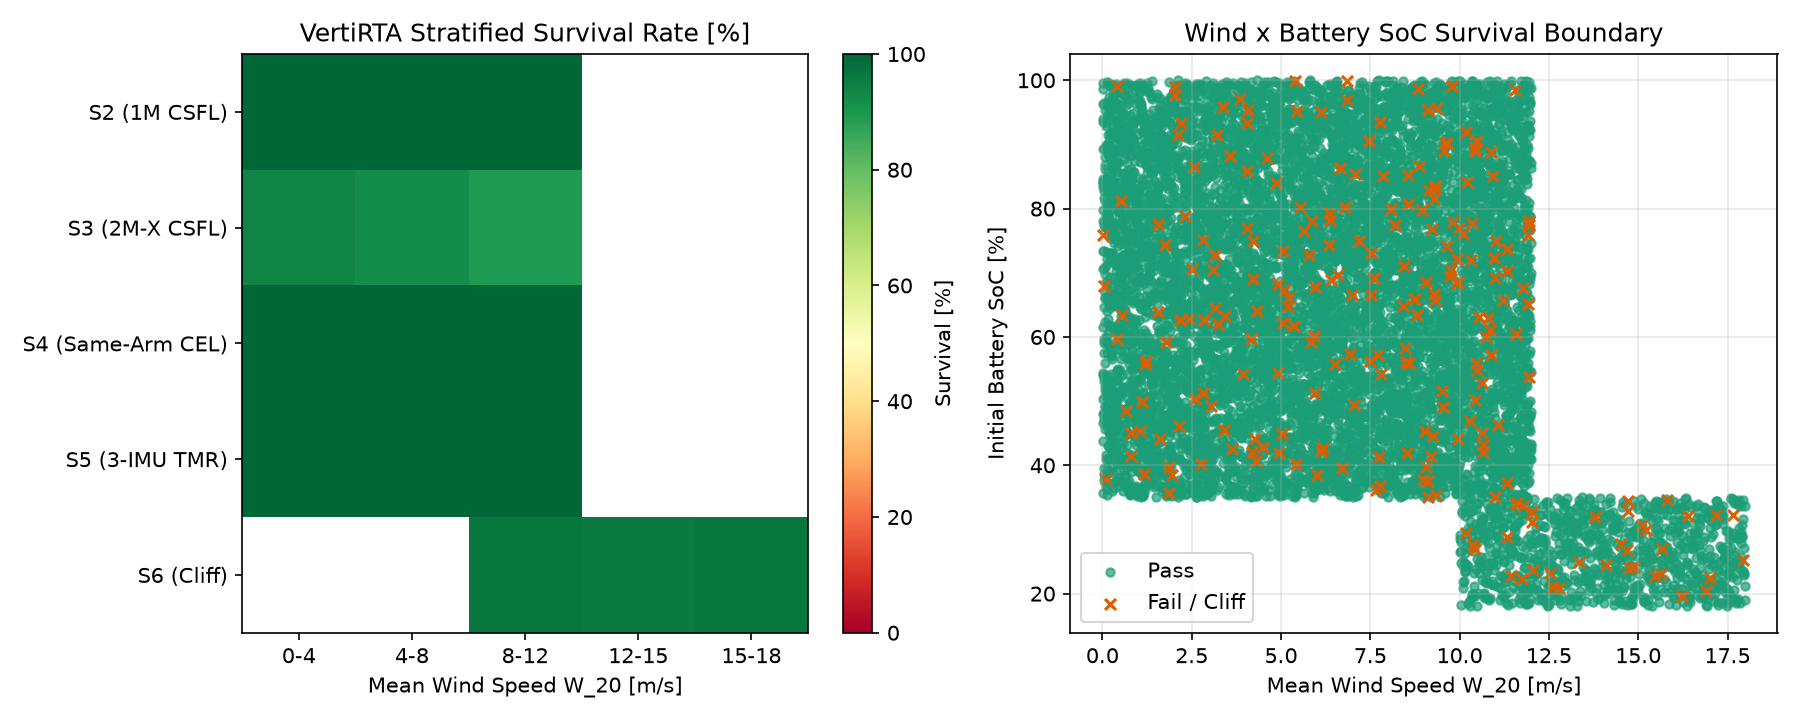
\includegraphics[width=\columnwidth]{../../artifacts/v1.0.0/tier1_atlas/survival_heatmap.png}
  \caption{Tier-1 10{,}000-run stratified 6-DOF survival envelope heatmap (\texttt{HJ-CBVF+INDI-WLS}) across coastal wind speed and initial pack SoC, highlighting genuine S3/S6 boundary cliffs rather than hiding failures.}
  \label{fig:heatmap}
\end{figure}

\begin{figure}[t]
  \centering
  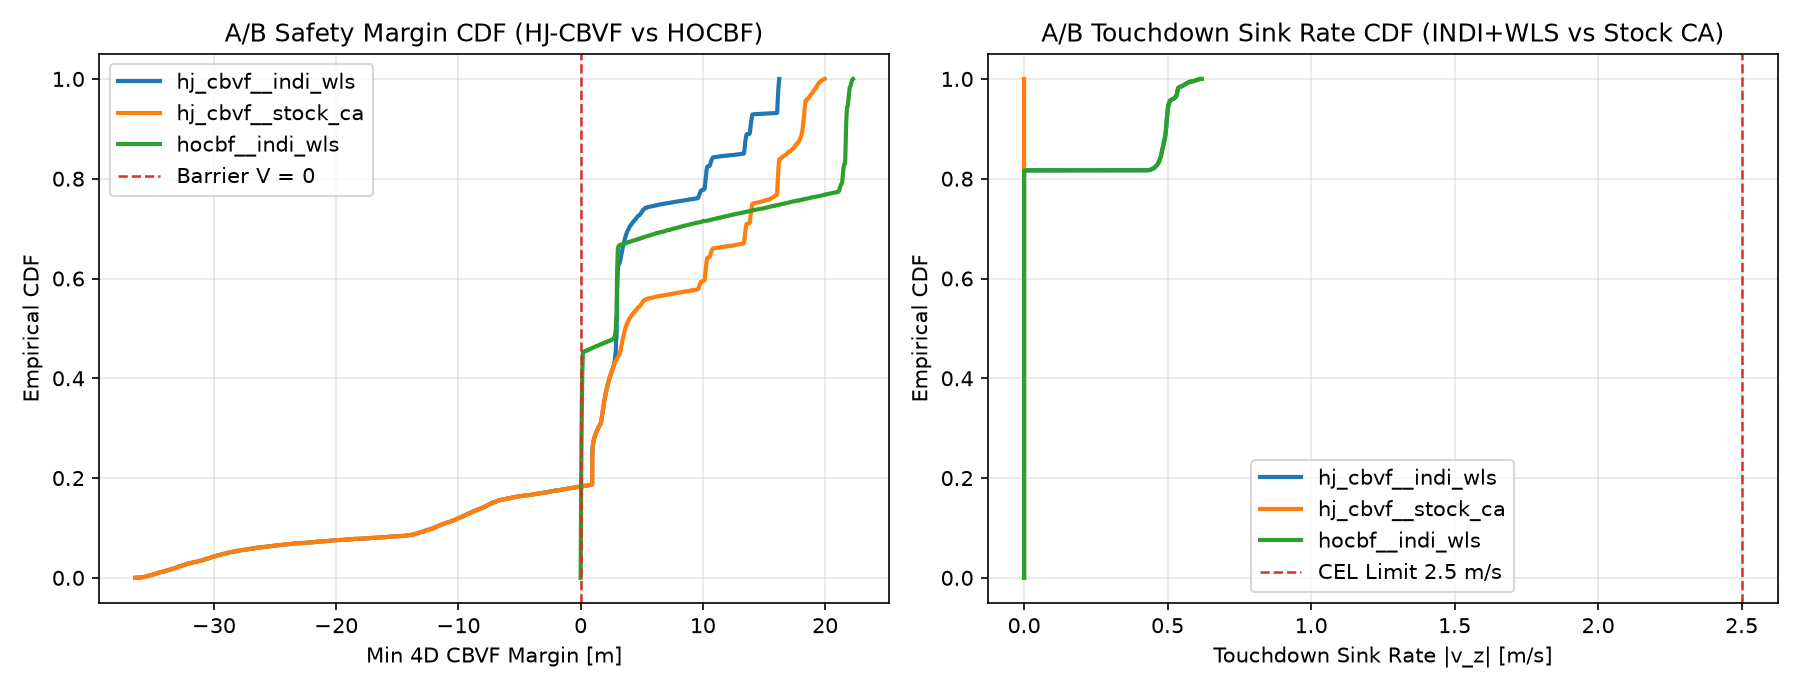
\includegraphics[width=\columnwidth]{../../artifacts/v1.0.0/tier1_atlas/ab_cdf.png}
  \caption{Empirical CDF comparison across the 30{,}000-simulation A/B ablation (\texttt{HJ-CBVF+INDI-WLS} vs.\ \texttt{HOCBF+INDI-WLS} vs.\ \texttt{HJ-CBVF+Stock CA}).}
  \label{fig:abcdf}
\end{figure}

\section{Regulatory Positioning and Living Safety Case}
\label{sec:reg}

Aviation systems engineers rightly scrutinize conflation of unmanned Specific-category and manned Certified-category rules. VertiRTA maintains a strict two-stage regulatory separation grounded in 2024--2026 EASA and SHGM frameworks~\cite{easa_scvtol_2024,eu_part_iam_2024,easa_sora25_2026,shgm_sht_iha_2026}:
\begin{itemize}
  \item \textbf{Stage-A (25\,kg Unmanned Subscale CONOPS):} Experimental unmanned flight testbed aligned with \texttt{SORA 2.5} (\texttt{ED Decision 2025/018/R} and \texttt{2026/010/R}, permanently retiring SORA~2.0 on 1~Jan~2027) over controlled or low-density airspace with strictly $0$ passengers.
  \item \textbf{Stage-B (240\,kg Urban UAM Reference):} Simulated architecture aligned with \texttt{SC-VTOL-02} Category Enhanced, \texttt{MOC-5}, and \texttt{Part-IAM} performance-based energy reserves, mapping in T\"urkiye to SHGM \texttt{SHT-\.IHA} class \texttt{M3} ($\ge 150$\,kg) with \texttt{\.IHATTYS} active geofencing.
\end{itemize}

Crucially, Monte Carlo simulation bounds only \emph{conditional} software recovery $P(\text{CSFL}\mid\text{fault, ODD})$ and can \emph{never} prove a $10^{-9}$/FH catastrophic probability target: via exact logarithmic inversion $\lceil\ln(0.05)/\ln(1-10^{-9})\rceil$ using \texttt{math.log1p}, establishing a 95\% upper bound below $10^{-9}$/FH with zero failures requires $2{,}995{,}732{,}273$ independent flight hours. Hardware reliability budgeting instead relies on SAE~ARP4761A fault-tree decomposition~\cite{sae_arp4761a_2023}. VertiRTA compiles its living safety case in SCSC-141C Goal Structuring Notation (GSN~v3)~\cite{scsc_gsn_v3_2021} via \texttt{verification/gsn/build\_gsn.py}, stamping live SHA-256 digests for verified artifacts (\texttt{Sn1}--\texttt{Sn4}, \texttt{Sn7}--\texttt{Sn10}), marking unexecuted PX4/Gazebo SITL solutions (\texttt{Sn5}, \texttt{Sn6}) explicitly pending, and programmatically locking physical hardware qualification (\texttt{G5}) and DO-178C/type-certification lifecycle (\texttt{G6}) as \texttt{[UNDEVELOPED]}.

\section{Reproducibility and Conclusion}
\label{sec:conclusion}

All tables in this manuscript are generated automatically from \texttt{docs/paper/metrics\_manifest.json} via \texttt{generate\_latex\_tables.py} and audited by \texttt{verify\_paper\_numbers.py} against placeholder drift, false certification phrasing, and number mismatches. The complete VertiRTA repository, Zenodo metadata (\texttt{.zenodo.json}), C++20/ROS~2 codebase, and \texttt{v1.0.0} evidence pack are released under Apache-2.0. Future execution on GitHub Actions \texttt{ubuntu-24.04-arm}, local PX4~v1.16/Gazebo Harmonic SITL, and Colab G4 Blackwell GPUs will populate the remaining explicitly marked pending entries without altering the underlying ASTM~F3269-21 safety isolation architecture.

\bibliographystyle{IEEEtran}
\bibliography{references}

\end{document}
